\documentclass[aspectratio=169]{beamer}
\usepackage[T1]{fontenc}
\usepackage[utf8]{inputenc}
\usepackage{lmodern}
\usepackage{microtype}
\usepackage{xcolor}
\usepackage{tikz}
\usetikzlibrary{positioning, arrows.meta, calc}
\usepackage{fontawesome5}

\definecolor{wurgreen}{HTML}{34B233}
\definecolor{darkgreen}{HTML}{1F6B1E}
\definecolor{darknavy}{HTML}{1A1A2E}
\definecolor{midgray}{HTML}{6B7280}
\definecolor{lightgray}{HTML}{F3F4F6}
\definecolor{lightgreen}{HTML}{E8F7E8}
\definecolor{bodytext}{HTML}{1F2937}
\definecolor{warnred}{HTML}{FEE2E2}
\definecolor{warnborder}{HTML}{EF4444}
\definecolor{codebg}{HTML}{1E1E2E}
\definecolor{codegreen}{HTML}{9ECE6A}
\definecolor{codeblue}{HTML}{7AA2F7}
\definecolor{codegray}{HTML}{C0CAF5}

\usetheme{default}
\usecolortheme{default}
\usefonttheme{professionalfonts}
\setbeamertemplate{navigation symbols}{}
\setbeamertemplate{itemize items}{\textcolor{wurgreen}{\textbullet}}
\setbeamertemplate{itemize subitem}{\textcolor{midgray}{--}}
\setbeamercolor{frametitle}{fg=white, bg=darknavy}
\setbeamerfont{frametitle}{size=\large, series=\bfseries}
\setbeamertemplate{frametitle}{%
  \begin{beamercolorbox}[wd=\paperwidth, ht=1.1cm, dp=0.2cm, leftskip=0.6cm]{frametitle}
    \usebeamerfont{frametitle}\insertframetitle
  \end{beamercolorbox}}
\setbeamercolor{background canvas}{bg=white}
\setbeamercolor{normal text}{fg=bodytext}
\setbeamertemplate{footline}{%
  \begin{beamercolorbox}[wd=\paperwidth, ht=0.4cm, dp=0.15cm]{footline}
    \hspace{0.5cm}\textcolor{midgray}{\tiny Introduction to Python · Module 0: Setting Up}%
    \hfill\textcolor{midgray}{\tiny \insertframenumber}\hspace{0.4cm}
  \end{beamercolorbox}}

\newcommand{\codebox}[1]{\begin{center}
  \begin{tikzpicture}
    \node[fill=codebg, rounded corners=4pt, inner sep=9pt, text width=0.85\textwidth, text=codegray]{%
      \ttfamily\small #1};
  \end{tikzpicture}\end{center}}

\begin{document}

% ── TITLE ──────────────────────────────────────────────────────────────────
{
\setbeamertemplate{footline}{}
\begin{frame}[plain]
  \begin{tikzpicture}[remember picture, overlay]
    \fill[darknavy] (current page.south west) rectangle (current page.north east);
    \fill[wurgreen] (current page.south west) rectangle
      ([xshift=0.45cm]current page.north west);
    \node[anchor=west, text=white, font=\huge\bfseries, text width=13cm]
      at ([xshift=1.1cm, yshift=1.4cm]current page.west)
      {Introduction to Python};
    \node[anchor=west, text=wurgreen, font=\large, text width=12cm]
      at ([xshift=1.1cm, yshift=0.2cm]current page.west)
      {Module 0 --- Setting Up Python};
    \node[anchor=west, text=midgray, font=\small, text width=12cm]
      at ([xshift=1.1cm, yshift=-1.3cm]current page.west)
      {Ways to run Python, editors \& IDEs, and virtual environments};
  \end{tikzpicture}
\end{frame}
}

% ── SLIDE 1: what is python ───────────────────────────────────────────────
\begin{frame}{What Is Python, Really?}
\vspace{0.2cm}
{\small \textbf{Python} is a programming language --- a way of writing instructions a computer
can follow. To \emph{run} those instructions, you need the \textbf{Python interpreter}: a
program that reads your code and executes it.}

\medskip
\begin{columns}[T]
  \column{0.48\textwidth}
  \vspace{0pt}
  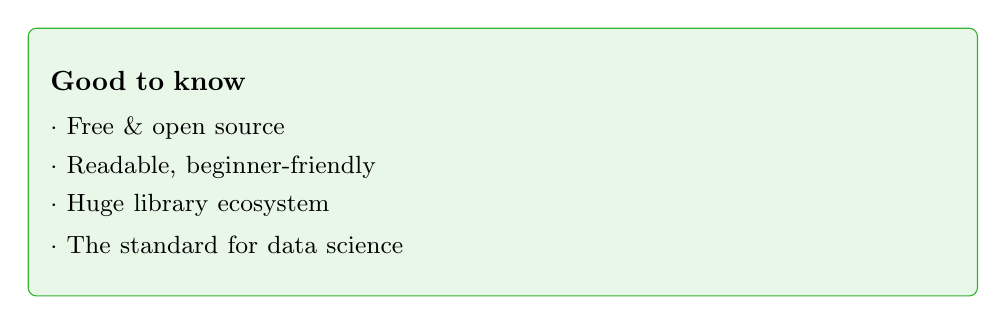
\begin{tikzpicture}
    \node[fill=lightgreen, draw=wurgreen, rounded corners=3pt,
          inner xsep=8pt, inner ysep=8pt, text width=\columnwidth-18pt, minimum height=3.4cm]{%
      \textbf{Good to know}\\[5pt]
      {\small
      $\cdot$ Free \& open source\\[3pt]
      $\cdot$ Readable, beginner-friendly\\[3pt]
      $\cdot$ Huge library ecosystem\\[3pt]
      $\cdot$ The standard for data science}};
  \end{tikzpicture}

  \column{0.48\textwidth}
  \vspace{0pt}
  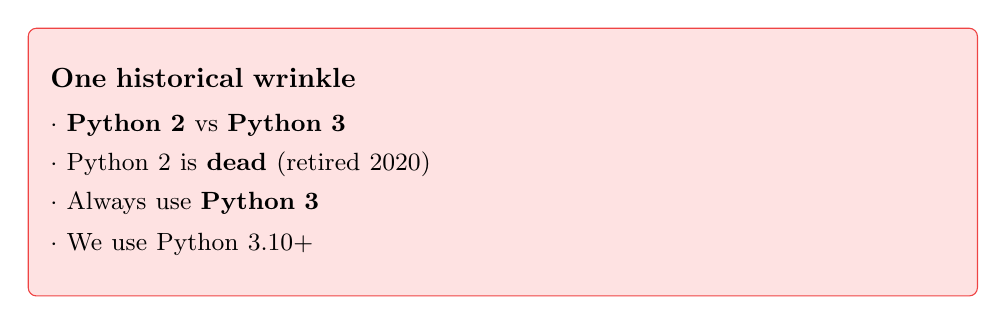
\begin{tikzpicture}
    \node[fill=warnred, draw=warnborder, rounded corners=3pt,
          inner xsep=8pt, inner ysep=8pt, text width=\columnwidth-18pt, minimum height=3.4cm]{%
      \textbf{One historical wrinkle}\\[5pt]
      {\small
      $\cdot$ \textbf{Python 2} vs \textbf{Python 3}\\[3pt]
      $\cdot$ Python 2 is \textbf{dead} (retired 2020)\\[3pt]
      $\cdot$ Always use \textbf{Python 3}\\[3pt]
      $\cdot$ We use Python 3.10+}};
  \end{tikzpicture}
\end{columns}

\medskip
{\small\textcolor{midgray}{\textit{You write \texttt{.py} files or notebook cells; the
interpreter turns them into actions.}}}
\end{frame}

% ── SLIDE 2: ways to run python ───────────────────────────────────────────
\begin{frame}{Three Ways to Run Python}
\vspace{0.2cm}
\begin{columns}[T]
  \column{0.32\textwidth}
  \vspace{0pt}
  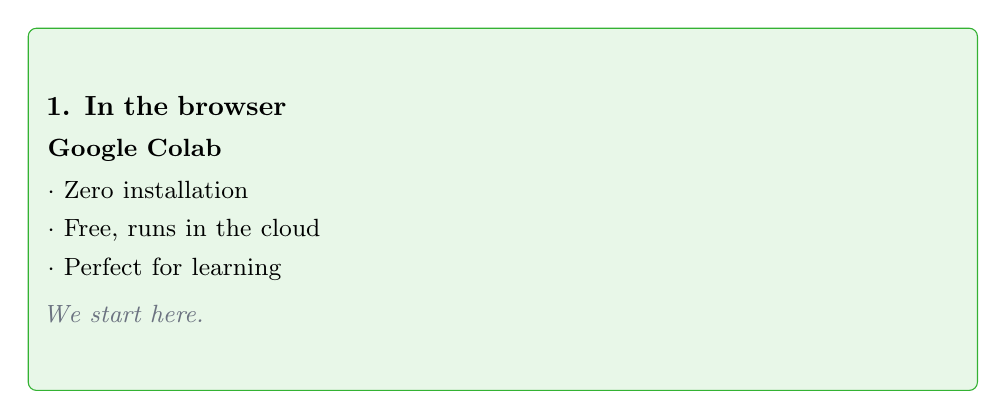
\begin{tikzpicture}
    \node[fill=lightgreen, draw=wurgreen, rounded corners=3pt,
          inner xsep=7pt, inner ysep=8pt, text width=\columnwidth-16pt, minimum height=4.6cm]{%
      \textbf{1. In the browser}\\[4pt]
      {\small \textbf{Google Colab}\\[4pt]
      $\cdot$ Zero installation\\[3pt]
      $\cdot$ Free, runs in the cloud\\[3pt]
      $\cdot$ Perfect for learning\\[5pt]
      \textcolor{midgray}{\textit{We start here.}}}};
  \end{tikzpicture}

  \column{0.32\textwidth}
  \vspace{0pt}
  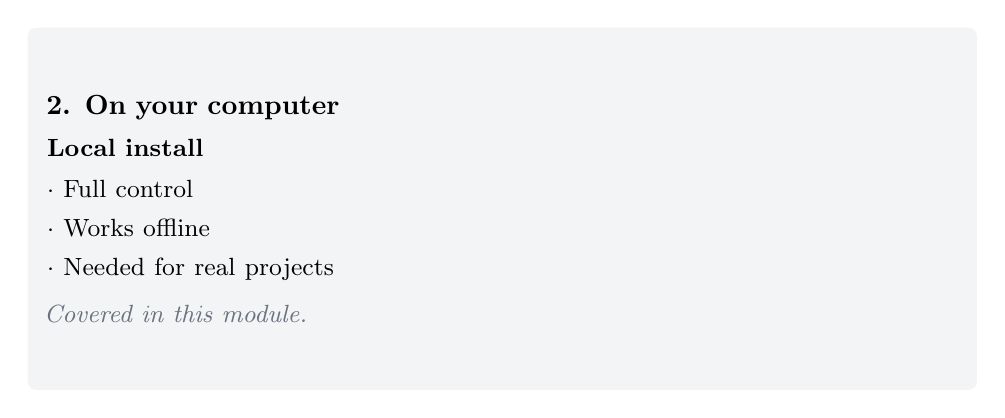
\begin{tikzpicture}
    \node[fill=lightgray, rounded corners=3pt,
          inner xsep=7pt, inner ysep=8pt, text width=\columnwidth-16pt, minimum height=4.6cm]{%
      \textbf{2. On your computer}\\[4pt]
      {\small \textbf{Local install}\\[4pt]
      $\cdot$ Full control\\[3pt]
      $\cdot$ Works offline\\[3pt]
      $\cdot$ Needed for real projects\\[5pt]
      \textcolor{midgray}{\textit{Covered in this module.}}}};
  \end{tikzpicture}

  \column{0.32\textwidth}
  \vspace{0pt}
  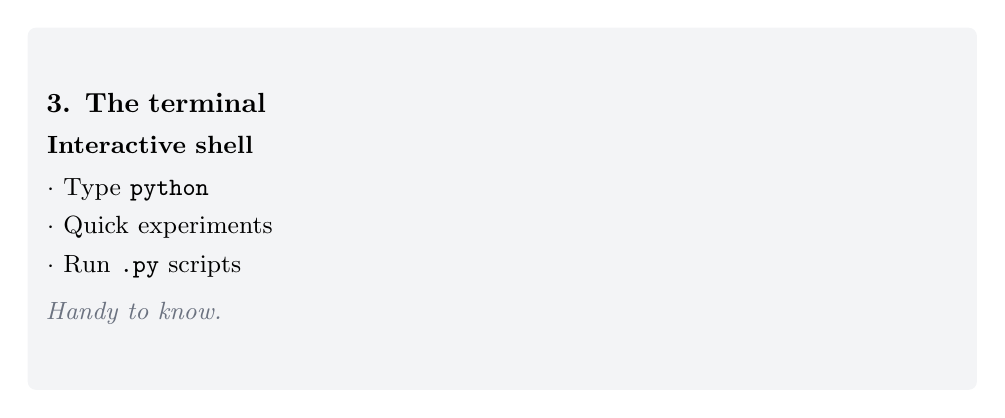
\begin{tikzpicture}
    \node[fill=lightgray, rounded corners=3pt,
          inner xsep=7pt, inner ysep=8pt, text width=\columnwidth-16pt, minimum height=4.6cm]{%
      \textbf{3. The terminal}\\[4pt]
      {\small \textbf{Interactive shell}\\[4pt]
      $\cdot$ Type \texttt{python}\\[3pt]
      $\cdot$ Quick experiments\\[3pt]
      $\cdot$ Run \texttt{.py} scripts\\[5pt]
      \textcolor{midgray}{\textit{Handy to know.}}}};
  \end{tikzpicture}
\end{columns}

\medskip
{\small\textcolor{midgray}{\textit{For this course, \textbf{Colab} is all you need. The rest of
this module is for when you set up Python on your \emph{own} machine.}}}
\end{frame}

% ── SLIDE 3: local install ────────────────────────────────────────────────
\begin{frame}{Installing Python Locally}
\vspace{0.2cm}
{\small Two common routes. Both work --- pick one.}

\medskip
\begin{columns}[T]
  \column{0.48\textwidth}
  \vspace{0pt}
  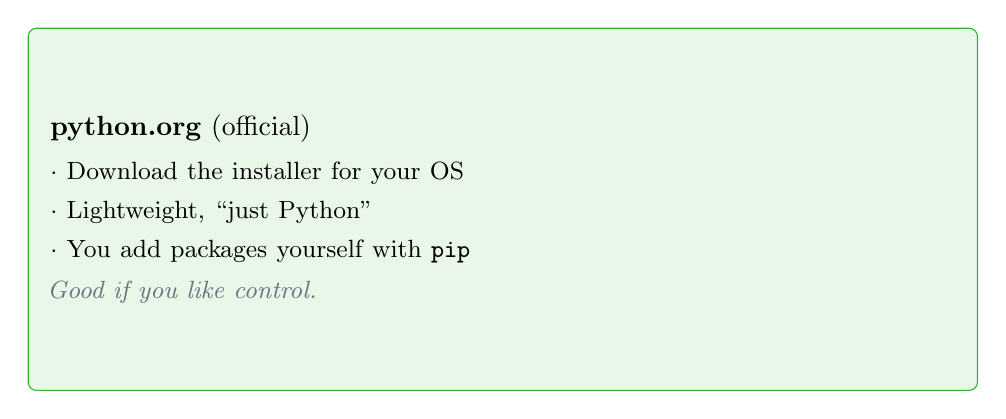
\begin{tikzpicture}
    \node[fill=lightgreen, draw=wurgreen, rounded corners=3pt,
          inner xsep=8pt, inner ysep=8pt, text width=\columnwidth-18pt, minimum height=4.6cm]{%
      \textbf{python.org} (official)\\[5pt]
      {\small
      $\cdot$ Download the installer for your OS\\[3pt]
      $\cdot$ Lightweight, ``just Python''\\[3pt]
      $\cdot$ You add packages yourself with \texttt{pip}\\[3pt]
      \textcolor{midgray}{\textit{Good if you like control.}}}};
  \end{tikzpicture}

  \column{0.48\textwidth}
  \vspace{0pt}
  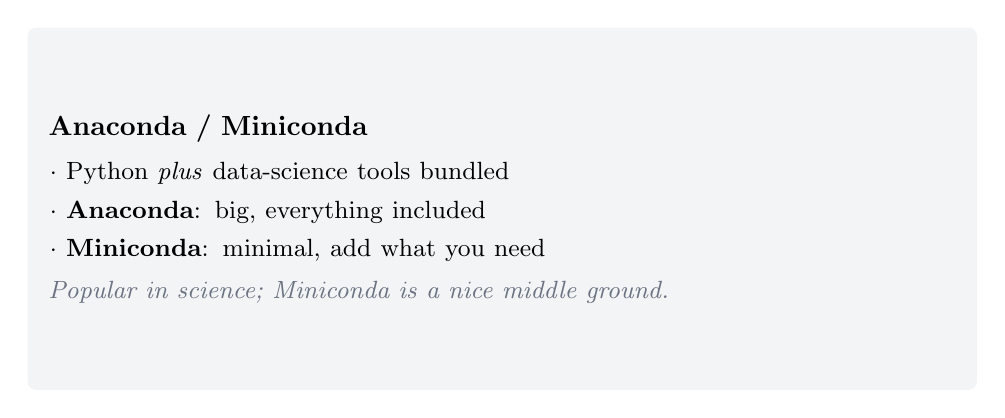
\begin{tikzpicture}
    \node[fill=lightgray, rounded corners=3pt,
          inner xsep=8pt, inner ysep=8pt, text width=\columnwidth-18pt, minimum height=4.6cm]{%
      \textbf{Anaconda / Miniconda}\\[5pt]
      {\small
      $\cdot$ Python \emph{plus} data-science tools bundled\\[3pt]
      $\cdot$ \textbf{Anaconda}: big, everything included\\[3pt]
      $\cdot$ \textbf{Miniconda}: minimal, add what you need\\[3pt]
      \textcolor{midgray}{\textit{Popular in science; Miniconda is a nice middle ground.}}}};
  \end{tikzpicture}
\end{columns}

\medskip
{\small\textcolor{midgray}{\textit{On Windows, tick ``Add Python to PATH'' during install ---
it saves a lot of headaches later.}}}
\end{frame}

% ── SLIDE 4: editors and IDEs ─────────────────────────────────────────────
\begin{frame}{Where You Write Code: Editors \& IDEs}
\vspace{0.2cm}
{\small An \textbf{IDE} (Integrated Development Environment) is a program for writing, running,
and debugging code. A few popular ones:}

\medskip
\begin{center}
\renewcommand{\arraystretch}{1.35}
{\small
\begin{tabular}{p{2.7cm}|p{9.3cm}}
\textbf{VS Code} & Free, lightweight, hugely popular. Great all-rounder --- our recommendation \\
\textbf{Jupyter / JupyterLab} & Notebook interface (like Colab, but local). Ideal for data analysis \\
\textbf{PyCharm} & Powerful, full-featured IDE. More for large software projects \\
\textbf{Spyder} & MATLAB-like; comes with Anaconda. Popular with scientists \\
\end{tabular}
}
\end{center}

\medskip
{\small\textcolor{midgray}{\textit{There is no single ``right'' one. For general Python work
we suggest \textbf{VS Code}; for data analysis, many people live in \textbf{notebooks}.}}}
\end{frame}

% ── SLIDE 5: VS Code walkthrough ──────────────────────────────────────────
\begin{frame}{Getting Started with VS Code}
\vspace{0.2cm}
{\small \textbf{VS Code} (Visual Studio Code) is a free editor from Microsoft. Setting it up
for Python takes a few steps:}

\medskip
\begin{columns}[T]
  \column{0.5\textwidth}
  \vspace{0pt}
  {\small
  \textcolor{wurgreen}{\textbf{1.}} Download from \texttt{code.visualstudio.com}\\[6pt]
  \textcolor{wurgreen}{\textbf{2.}} Install the \textbf{Python extension} (from the Extensions panel)\\[6pt]
  \textcolor{wurgreen}{\textbf{3.}} Open a folder for your project\\[6pt]
  \textcolor{wurgreen}{\textbf{4.}} Create a \texttt{.py} file and start writing}

  \column{0.5\textwidth}
  \vspace{0pt}
  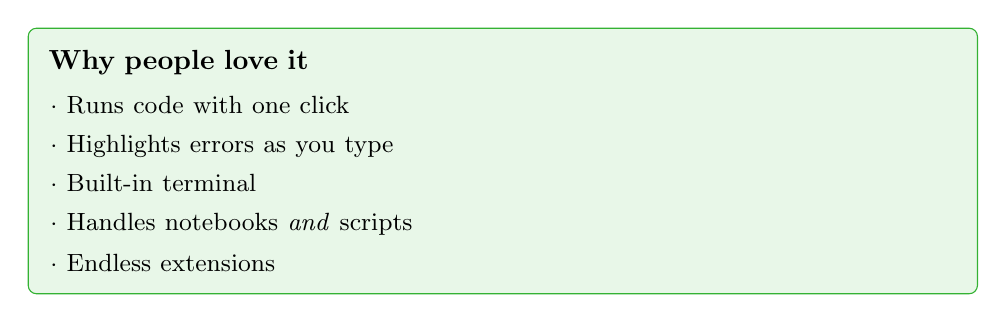
\begin{tikzpicture}
    \node[fill=lightgreen, draw=wurgreen, rounded corners=3pt,
          inner xsep=8pt, inner ysep=8pt, text width=\columnwidth-18pt]{%
      \textbf{Why people love it}\\[5pt]
      {\small
      $\cdot$ Runs code with one click\\[3pt]
      $\cdot$ Highlights errors as you type\\[3pt]
      $\cdot$ Built-in terminal\\[3pt]
      $\cdot$ Handles notebooks \emph{and} scripts\\[3pt]
      $\cdot$ Endless extensions}};
  \end{tikzpicture}
\end{columns}

\medskip
{\small\textcolor{midgray}{\textit{VS Code can also open \texttt{.ipynb} notebooks directly ---
so you get the best of both worlds.}}}
\end{frame}

% ── SLIDE 6: why virtual environments ─────────────────────────────────────
\begin{frame}{Virtual Environments: The Why}
\vspace{0.2cm}
{\small Here is a problem you \emph{will} hit. Project A needs version 1 of a library; project B
needs version 2. Install them globally and they \textbf{clash}.}

\medskip
\begin{center}
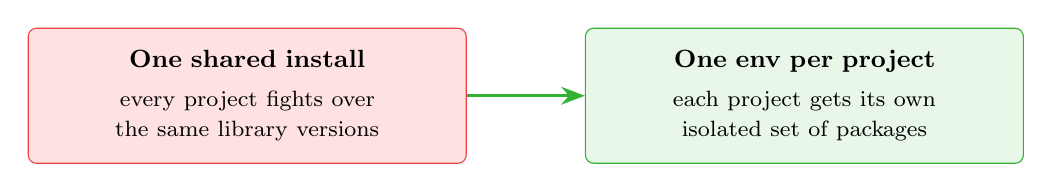
\begin{tikzpicture}[font=\small]
  \node[fill=warnred, draw=warnborder, rounded corners=3pt, inner sep=8pt, text width=5cm, align=center] (bad)
    {\textbf{One shared install}\\[3pt]{\footnotesize every project fights over the same library versions}};
  \node[fill=lightgreen, draw=wurgreen, rounded corners=3pt, inner sep=8pt,
        text width=5cm, align=center, right=1.5cm of bad] (good)
    {\textbf{One env per project}\\[3pt]{\footnotesize each project gets its own isolated set of packages}};
  \draw[-{Stealth[length=3mm]}, wurgreen, line width=1.2pt] (bad) -- (good);
\end{tikzpicture}
\end{center}

\medskip
{\small A \textbf{virtual environment} is an isolated Python setup for a single project. Its
packages live in their own folder and don't interfere with anything else. \textbf{Use one per
project} --- it is the single best habit you can build early.}
\end{frame}

% ── SLIDE 7: virtual environments - venv ──────────────────────────────────
\begin{frame}{Virtual Environments: The How (\texttt{venv})}
\vspace{0.2cm}
{\small Python's built-in tool is \texttt{venv}. In a terminal, inside your project folder:}

\medskip
\codebox{%
\textcolor{codegray}{\# create an environment called ".venv"}\\
python -m venv .venv\\[6pt]
\textcolor{codegray}{\# activate it (Mac/Linux)}\\
\textcolor{codeblue}{source} .venv/bin/activate\\[6pt]
\textcolor{codegray}{\# activate it (Windows)}\\
.venv\textbackslash Scripts\textbackslash activate\\[6pt]
\textcolor{codegray}{\# now install packages -- they go inside .venv only}\\
pip \textcolor{codeblue}{install} pandas numpy}

\medskip
{\small When activated, your prompt shows \texttt{(.venv)}. Type \texttt{deactivate} to leave.
Everything you \texttt{pip install} while active stays \textbf{inside} this environment.}
\end{frame}

% ── SLIDE 8: conda + requirements ─────────────────────────────────────────
\begin{frame}{Conda \& Sharing Your Setup}
\vspace{0.2cm}
\begin{columns}[T]
  \column{0.48\textwidth}
  \vspace{0pt}
  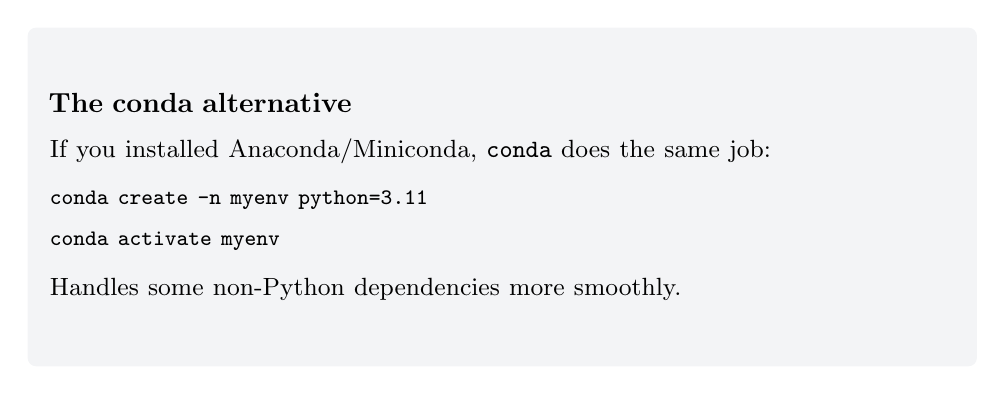
\begin{tikzpicture}
    \node[fill=lightgray, rounded corners=3pt,
          inner xsep=8pt, inner ysep=8pt, text width=\columnwidth-18pt, minimum height=4.3cm]{%
      \textbf{The conda alternative}\\[5pt]
      {\small If you installed Anaconda/Miniconda, \texttt{conda} does the same job:\\[6pt]
      \texttt{\footnotesize conda create -n myenv python=3.11}\\[4pt]
      \texttt{\footnotesize conda activate myenv}\\[6pt]
      Handles some non-Python dependencies more smoothly.}};
  \end{tikzpicture}

  \column{0.48\textwidth}
  \vspace{0pt}
  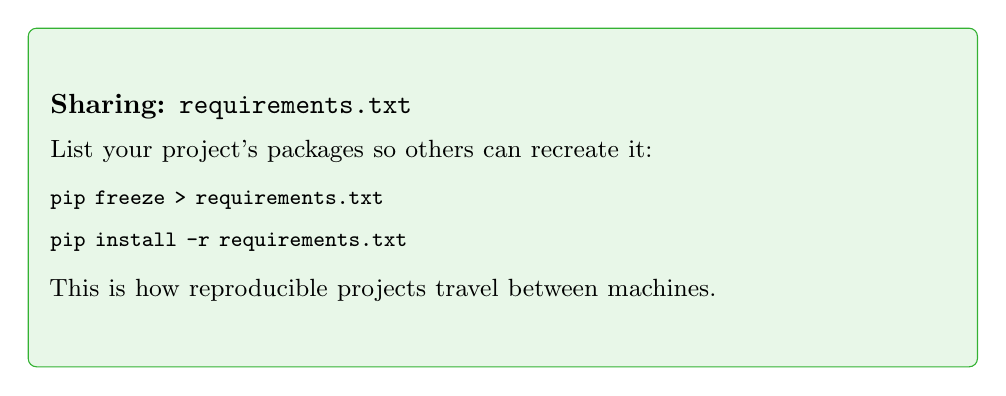
\begin{tikzpicture}
    \node[fill=lightgreen, draw=wurgreen, rounded corners=3pt,
          inner xsep=8pt, inner ysep=8pt, text width=\columnwidth-18pt, minimum height=4.3cm]{%
      \textbf{Sharing: \texttt{requirements.txt}}\\[5pt]
      {\small List your project's packages so others can recreate it:\\[6pt]
      \texttt{\footnotesize pip freeze > requirements.txt}\\[4pt]
      \texttt{\footnotesize pip install -r requirements.txt}\\[6pt]
      This is how reproducible projects travel between machines.}};
  \end{tikzpicture}
\end{columns}

\medskip
{\small\textcolor{midgray}{\textit{\texttt{venv} + \texttt{pip} or \texttt{conda} --- either is
fine. The key idea is the same: \textbf{isolate, then record}.}}}
\end{frame}

% ── SLIDE: what is git/github/cloning ─────────────────────────────────────
\begin{frame}{Getting Code from GitHub: Cloning}
\vspace{0.2cm}
{\small Course materials, shared projects, and most open-source code live on \textbf{GitHub}.
To get a copy onto your own machine, you \textbf{clone} the repository.}

\medskip
\begin{columns}[T]
  \column{0.48\textwidth}
  \vspace{0pt}
  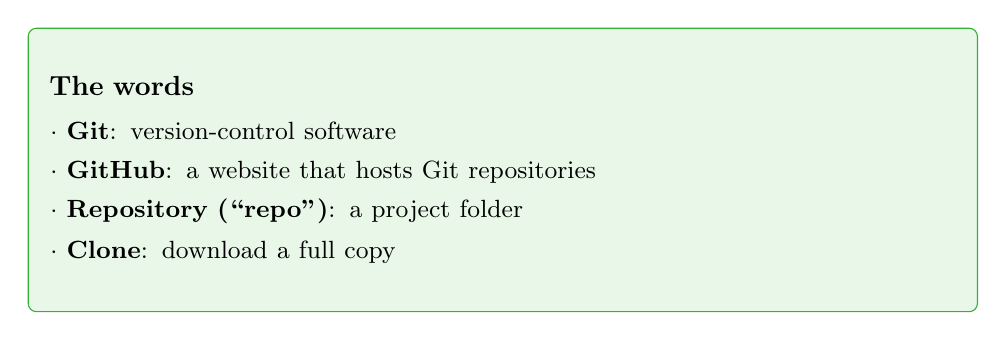
\begin{tikzpicture}
    \node[fill=lightgreen, draw=wurgreen, rounded corners=3pt,
          inner xsep=8pt, inner ysep=8pt, text width=\columnwidth-18pt, minimum height=3.6cm]{%
      \textbf{The words}\\[5pt]
      {\small
      $\cdot$ \textbf{Git}: version-control software\\[3pt]
      $\cdot$ \textbf{GitHub}: a website that hosts Git repositories\\[3pt]
      $\cdot$ \textbf{Repository (``repo'')}: a project folder\\[3pt]
      $\cdot$ \textbf{Clone}: download a full copy}};
  \end{tikzpicture}

  \column{0.48\textwidth}
  \vspace{0pt}
  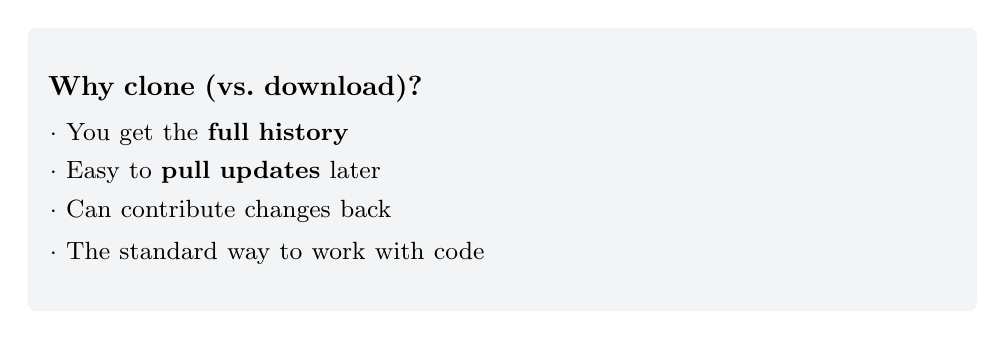
\begin{tikzpicture}
    \node[fill=lightgray, rounded corners=3pt,
          inner xsep=8pt, inner ysep=8pt, text width=\columnwidth-18pt, minimum height=3.6cm]{%
      \textbf{Why clone (vs.\ download)?}\\[5pt]
      {\small
      $\cdot$ You get the \textbf{full history}\\[3pt]
      $\cdot$ Easy to \textbf{pull updates} later\\[3pt]
      $\cdot$ Can contribute changes back\\[3pt]
      $\cdot$ The standard way to work with code}};
  \end{tikzpicture}
\end{columns}

\medskip
{\small\textcolor{midgray}{\textit{You only need the repository's URL --- found on its GitHub page
under the green ``Code'' button.}}}
\end{frame}

% ── SLIDE: ways to clone ──────────────────────────────────────────────────
\begin{frame}{Four Ways to Clone a Repository}
\vspace{0.15cm}
{\small \textbf{1. The terminal} (the classic way) --- \texttt{cd} into where you want it, then:}
\smallskip
\codebox{git \textcolor{codeblue}{clone} https://github.com/username/repo-name.git}

\smallskip
{\small \textbf{2. GitHub Desktop} --- a friendly app, no terminal. \emph{File $\rightarrow$ Clone
Repository}, paste the URL, pick a folder. Great for beginners.}

\smallskip
{\small \textbf{3. VS Code} --- built in. Open the Command Palette
(\texttt{Ctrl/Cmd+Shift+P}), type \emph{``Git: Clone''}, paste the URL.}

\smallskip
{\small \textbf{4. Download ZIP} (not really cloning) --- the green \textbf{Code} button
$\rightarrow$ \emph{Download ZIP}. Quick, but you lose history and can't easily pull updates.}

\medskip
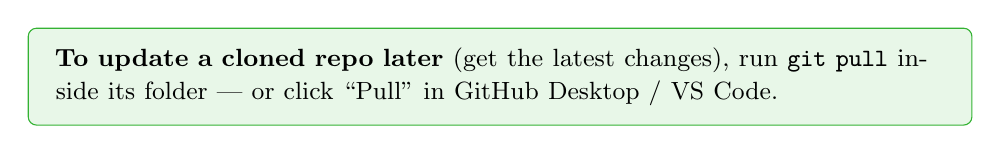
\begin{tikzpicture}
  \node[fill=lightgreen, draw=wurgreen, rounded corners=3pt,
        inner xsep=10pt, inner ysep=7pt, text width=\textwidth-24pt]{%
    {\small \textbf{To update a cloned repo later} (get the latest changes), run
    \texttt{git pull} inside its folder --- or click ``Pull'' in GitHub Desktop / VS Code.}};
\end{tikzpicture}
\end{frame}

% ── SLIDE 9: recap ────────────────────────────────────────────────────────
\begin{frame}{Module 0: Takeaways}
\vspace{0.25cm}
\begin{itemize}\setlength\itemsep{8pt}
  \item[\textcolor{wurgreen}{\faCheck}]
    Python is a language; the \textbf{interpreter} runs it --- always use \textbf{Python 3}
  \item[\textcolor{wurgreen}{\faCheck}]
    Run it in \textbf{Colab} (easiest), a \textbf{local install}, or the \textbf{terminal}
  \item[\textcolor{wurgreen}{\faCheck}]
    Write code in an \textbf{IDE} --- \textbf{VS Code} is a great default; notebooks suit data work
  \item[\textcolor{wurgreen}{\faCheck}]
    Use a \textbf{virtual environment per project} (\texttt{venv} or \texttt{conda}) to avoid
    version clashes
  \item[\textcolor{wurgreen}{\faCheck}]
    Record your packages in \textbf{\texttt{requirements.txt}} for reproducibility
  \item[\textcolor{wurgreen}{\faCheck}]
    \textbf{Clone} a GitHub repo (terminal, GitHub Desktop, VS Code) to get code onto your machine
  \item[\textcolor{wurgreen}{\faCheck}]
    \textbf{For this course, Colab is enough} --- come back here when you go local
\end{itemize}

\medskip
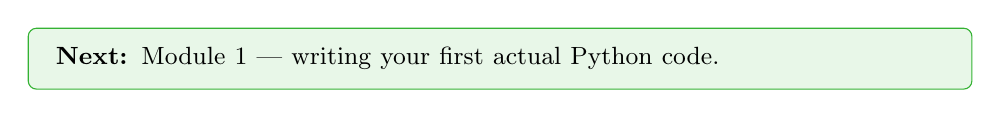
\begin{tikzpicture}
  \node[fill=lightgreen, draw=wurgreen, rounded corners=3pt,
        inner xsep=10pt, inner ysep=7pt, text width=\textwidth-24pt]{%
    {\small \textbf{Next:} Module 1 --- writing your first actual Python code.}};
\end{tikzpicture}
\end{frame}

\end{document}
